\url{https://github.com/cedrict/fieldstone/tree/master/python_codes/fieldstone_54}

\vspace{1cm}

This stone implements three different free surface/mesh deformation algorithms. 
The first one has all the nodes move with the computed velocity (Lagrangian method)
and is coined 'method 1'. 
The second one ('method 2') only has the top row of nodes moving with the computed velocity, 
while all the nodes underneath are static (this is obviously not a viable method for 
large deformations). 
The third one ('method 3') is the method used in ASPECT and described in Rose et al (2017) \cite{robh17}.
Its implementation is described in Section~\ref{sec:freesurface}.

Note that at the moment, and for all three methods, the movement of the surface nodes is limited 
to the vertical direction!

The domain is a 2D Cartesian box of size 512$\times$512km, with free slip on left, 
bottom and right sides, free surface at the top. 
Mantle material characterised by $\rho_m=3200$ and $\eta_m=10^{21}$. 
Gravity is vertical and Earth like. 
The surface is perturbed at startup by $\delta y = A \cos (\pi x /L_x)$ with $A$=1km.
200 time steps with $\delta t=10$kyr are carried out.
The root mean square velocity, the total volume of the domain, the min/max elevation
values of the surface are recorded over time. 

\begin{center}
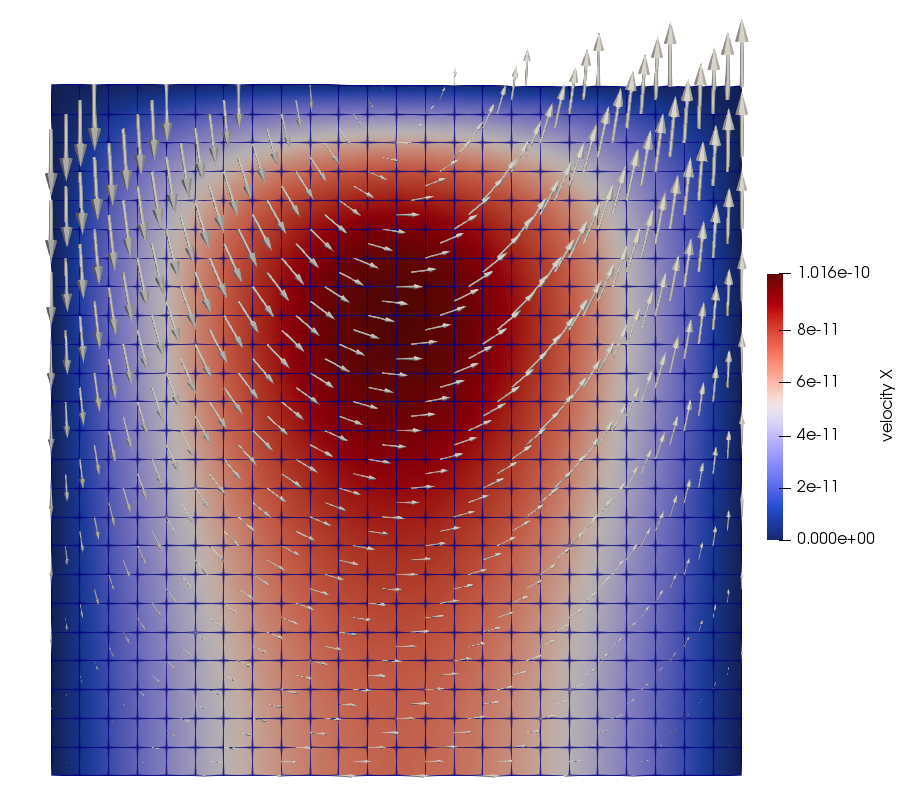
\includegraphics[width=7.5cm]{python_codes/fieldstone_54/images/u}
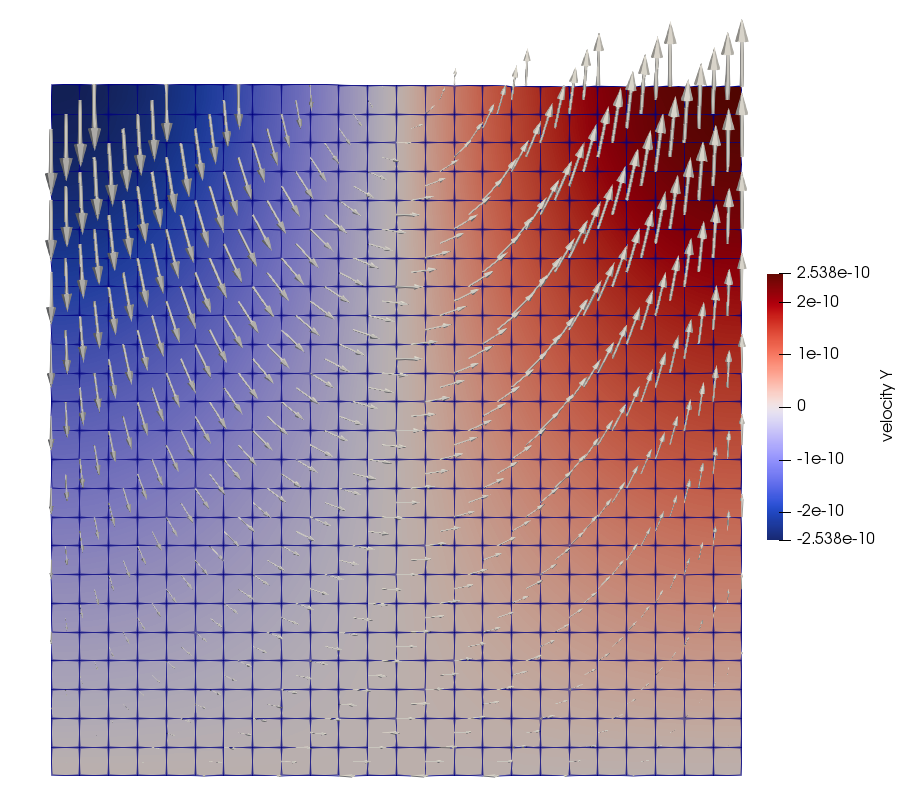
\includegraphics[width=7.5cm]{python_codes/fieldstone_54/images/v}\\
{\scriptsize velocity field at $t=0$ with resolution 24x24}
\end{center}

The results hereunder are obtained for all three methods at two different resolutions (16x16 
and 24x24 elements).
The plots on the left column are obtained with the movement of the top nodes being constrained in 
the vertical direction, while the plots on the right column are obtained with nodes being 
allowed to move in both $x$ and $y$ directions (note that for method 3 the normals are not -yet-
computed with the method of Eq. 49 in \cite{robh17} but instead by a simple geometric rule).

\begin{center}
a) 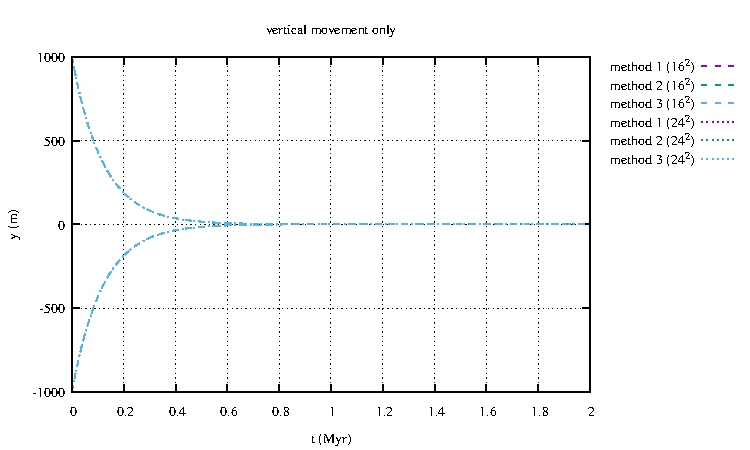
\includegraphics[width=7cm]{python_codes/fieldstone_54/images/elevation_vert.pdf}
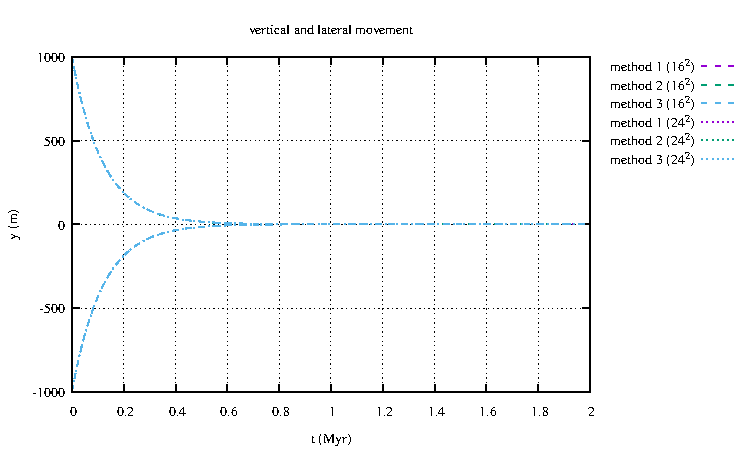
\includegraphics[width=7cm]{python_codes/fieldstone_54/images/elevation_full.pdf}\\
b) 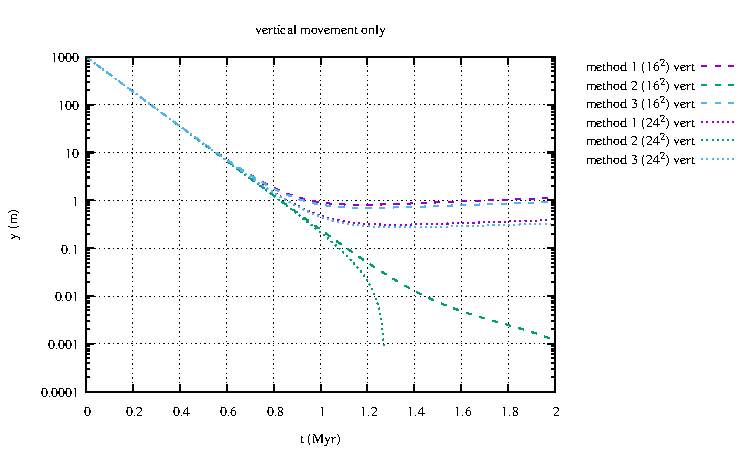
\includegraphics[width=7cm]{python_codes/fieldstone_54/images/elevation_log_vert.pdf}
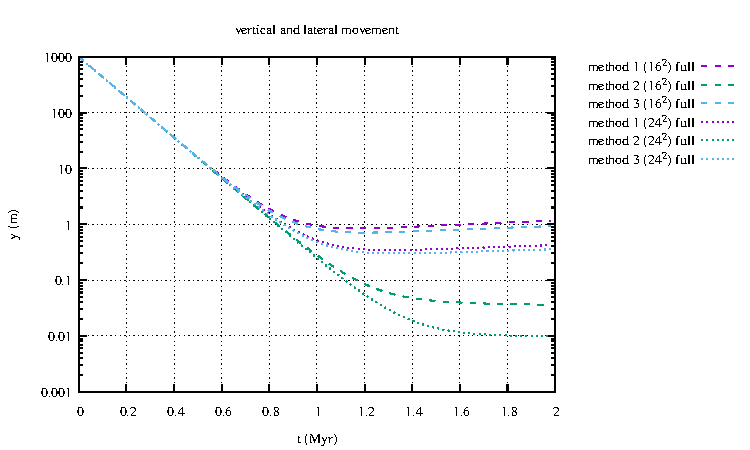
\includegraphics[width=7cm]{python_codes/fieldstone_54/images/elevation_log_full.pdf}\\
c) 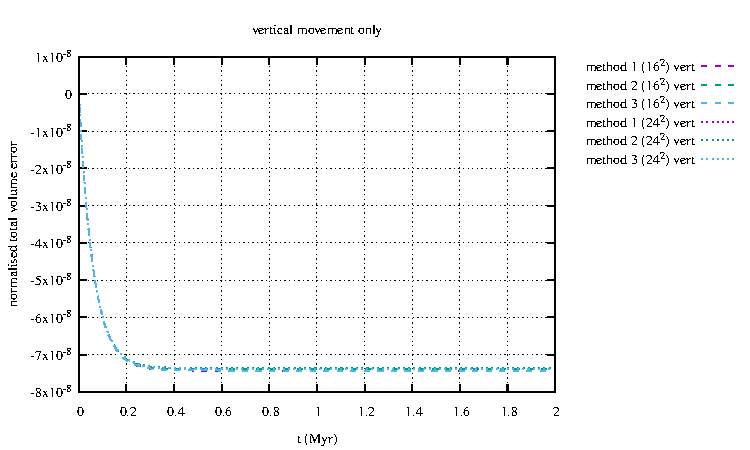
\includegraphics[width=7cm]{python_codes/fieldstone_54/images/volume_vert.pdf}
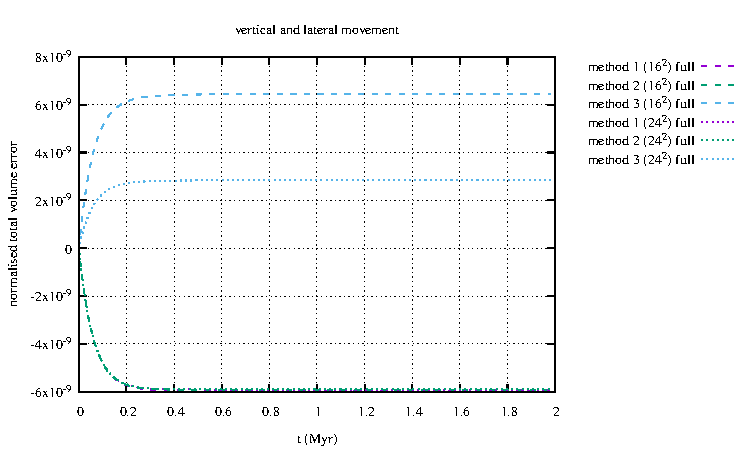
\includegraphics[width=7cm]{python_codes/fieldstone_54/images/volume_full.pdf}\\
d) 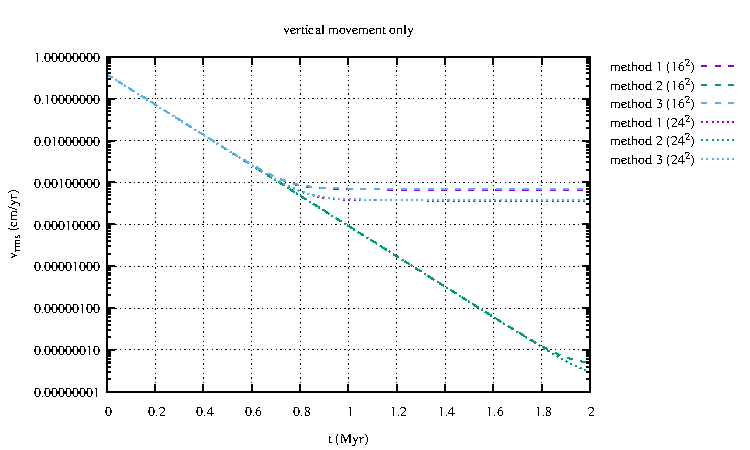
\includegraphics[width=7cm]{python_codes/fieldstone_54/images/vrms_vert.pdf}
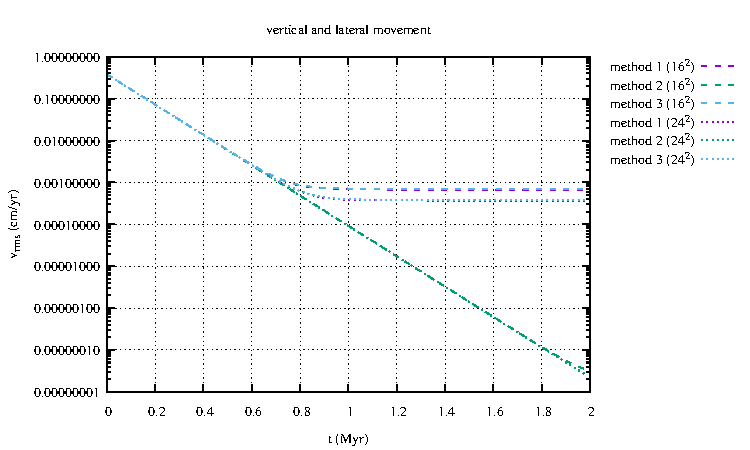
\includegraphics[width=7cm]{python_codes/fieldstone_54/images/vrms_full.pdf}\\
e) 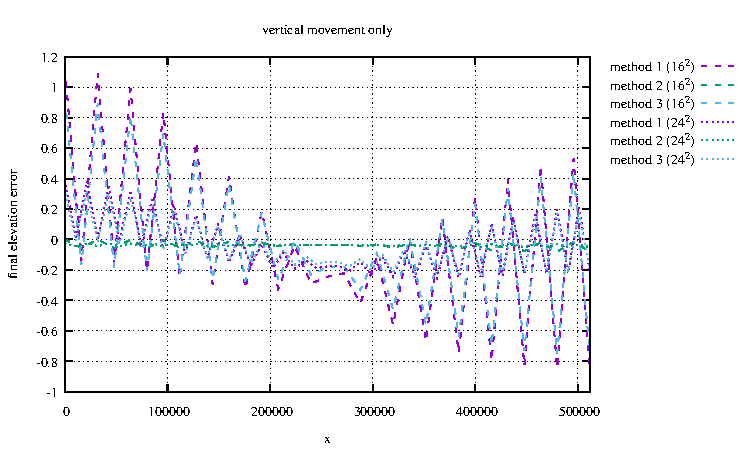
\includegraphics[width=7cm]{python_codes/fieldstone_54/images/surface_topography_200_vert.pdf}
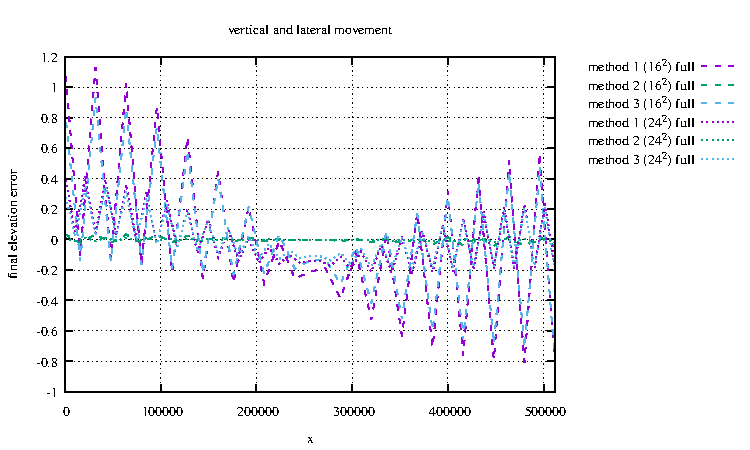
\includegraphics[width=7cm]{python_codes/fieldstone_54/images/surface_topography_200_full.pdf}\\
{\scriptsize 
a) min/max of free surface topo as a function of time; 
b) free surface topo maximum (in log scale) as a function of time; 
c) measured volume of the domain with numerical quadrature normalised by the expected volume $L_xL_y$;
d) root mean square velocity as a function of time;
e) final elevation at the 200th time step.}
\end{center}
